% !TEX root = ../../技术文档.tex
\section{图像采集与显示链路仿真验证}

本节包括采集重新使能、显示槽所有权、共享DDR背压和采显联合四类系统场景，以及紧凑显示组件回归。
前四类场景采用独立Video组件配置，采集通路包含原图、预览图和模型输入三路。
测试台在Windows原生ModelSim中运行，接口响应由可背压数字模型给出，所有比较均由测试台自检完成。
前四类场景的回归日志、WLF/VCD、输入哈希和原始仿真截图由\path{docs/verification/video/evidence/video_high_value_waveforms_20261030.json}统一登记。

\subsection{四类系统级场景}

表\ref{tbl:video-high-value-sim}给出短场景波形对应的通过统计。短场景用于保留关键事件的原始仿真波形，完整通过结果仍由同一测试入口的回归日志核对。

\begin{reporttable}
\begin{longtable}{@{}p{0.19\linewidth}p{0.24\linewidth}p{0.40\linewidth}p{0.10\linewidth}@{}}
\caption{Video链路高价值系统级仿真结果}\label{tbl:video-high-value-sim}\\
\toprule
场景 & 测试顶层 & 关键检查 & 结果 \\
\midrule
\endfirsthead
\caption[]{Video链路高价值系统级仿真结果（续）}\\
\toprule
场景 & 测试顶层 & 关键检查 & 结果 \\
\midrule
\endhead
\bottomrule
\endfoot
采集重新使能 & \texttt{capture\_\allowbreak rearm} & 7次采集成功、7次重新使能，三路写入共18522字节；完成响应排空后才发布完成事件 & PASS \\
显示槽所有权 & \texttt{slot\_\allowbreak owner} & 128位状态检查155项；提交、实际生效、代次、RETIRING、释放确认和空槽位图顺序一致 & PASS \\
共享DDR背压 & \texttt{memory\_\allowbreak scheduler} & 12次读、12次写；读写最大等待均为0，调度配额为4，故障保持为0 & PASS \\
采显联合 & \texttt{shared\_\allowbreak memory} & 7个任务、7800个像素、13次光栅；读写竞争重叠11690拍，读授权262次、写授权441次，欠载0 & PASS \\
\end{longtable}
\end{reporttable}

\subsection{采集与槽所有权}

采集波形中，\texttt{req\_\allowbreak valid}/\texttt{req\_\allowbreak ready}的握手先锁存帧号和槽号。
三路写入计数\texttt{raw\_\allowbreak written\_\allowbreak bytes}、
\texttt{preview\_\allowbreak written\_\allowbreak bytes}和\texttt{input\_\allowbreak written\_\allowbreak bytes}逐步增加；\texttt{port\_\allowbreak drained}置位后才出现
\texttt{completion\_\allowbreak valid}。成功场景中\texttt{error}保持为零，重新使能次数与成功次数相等。

\begin{figure}[!htbp]
\centering
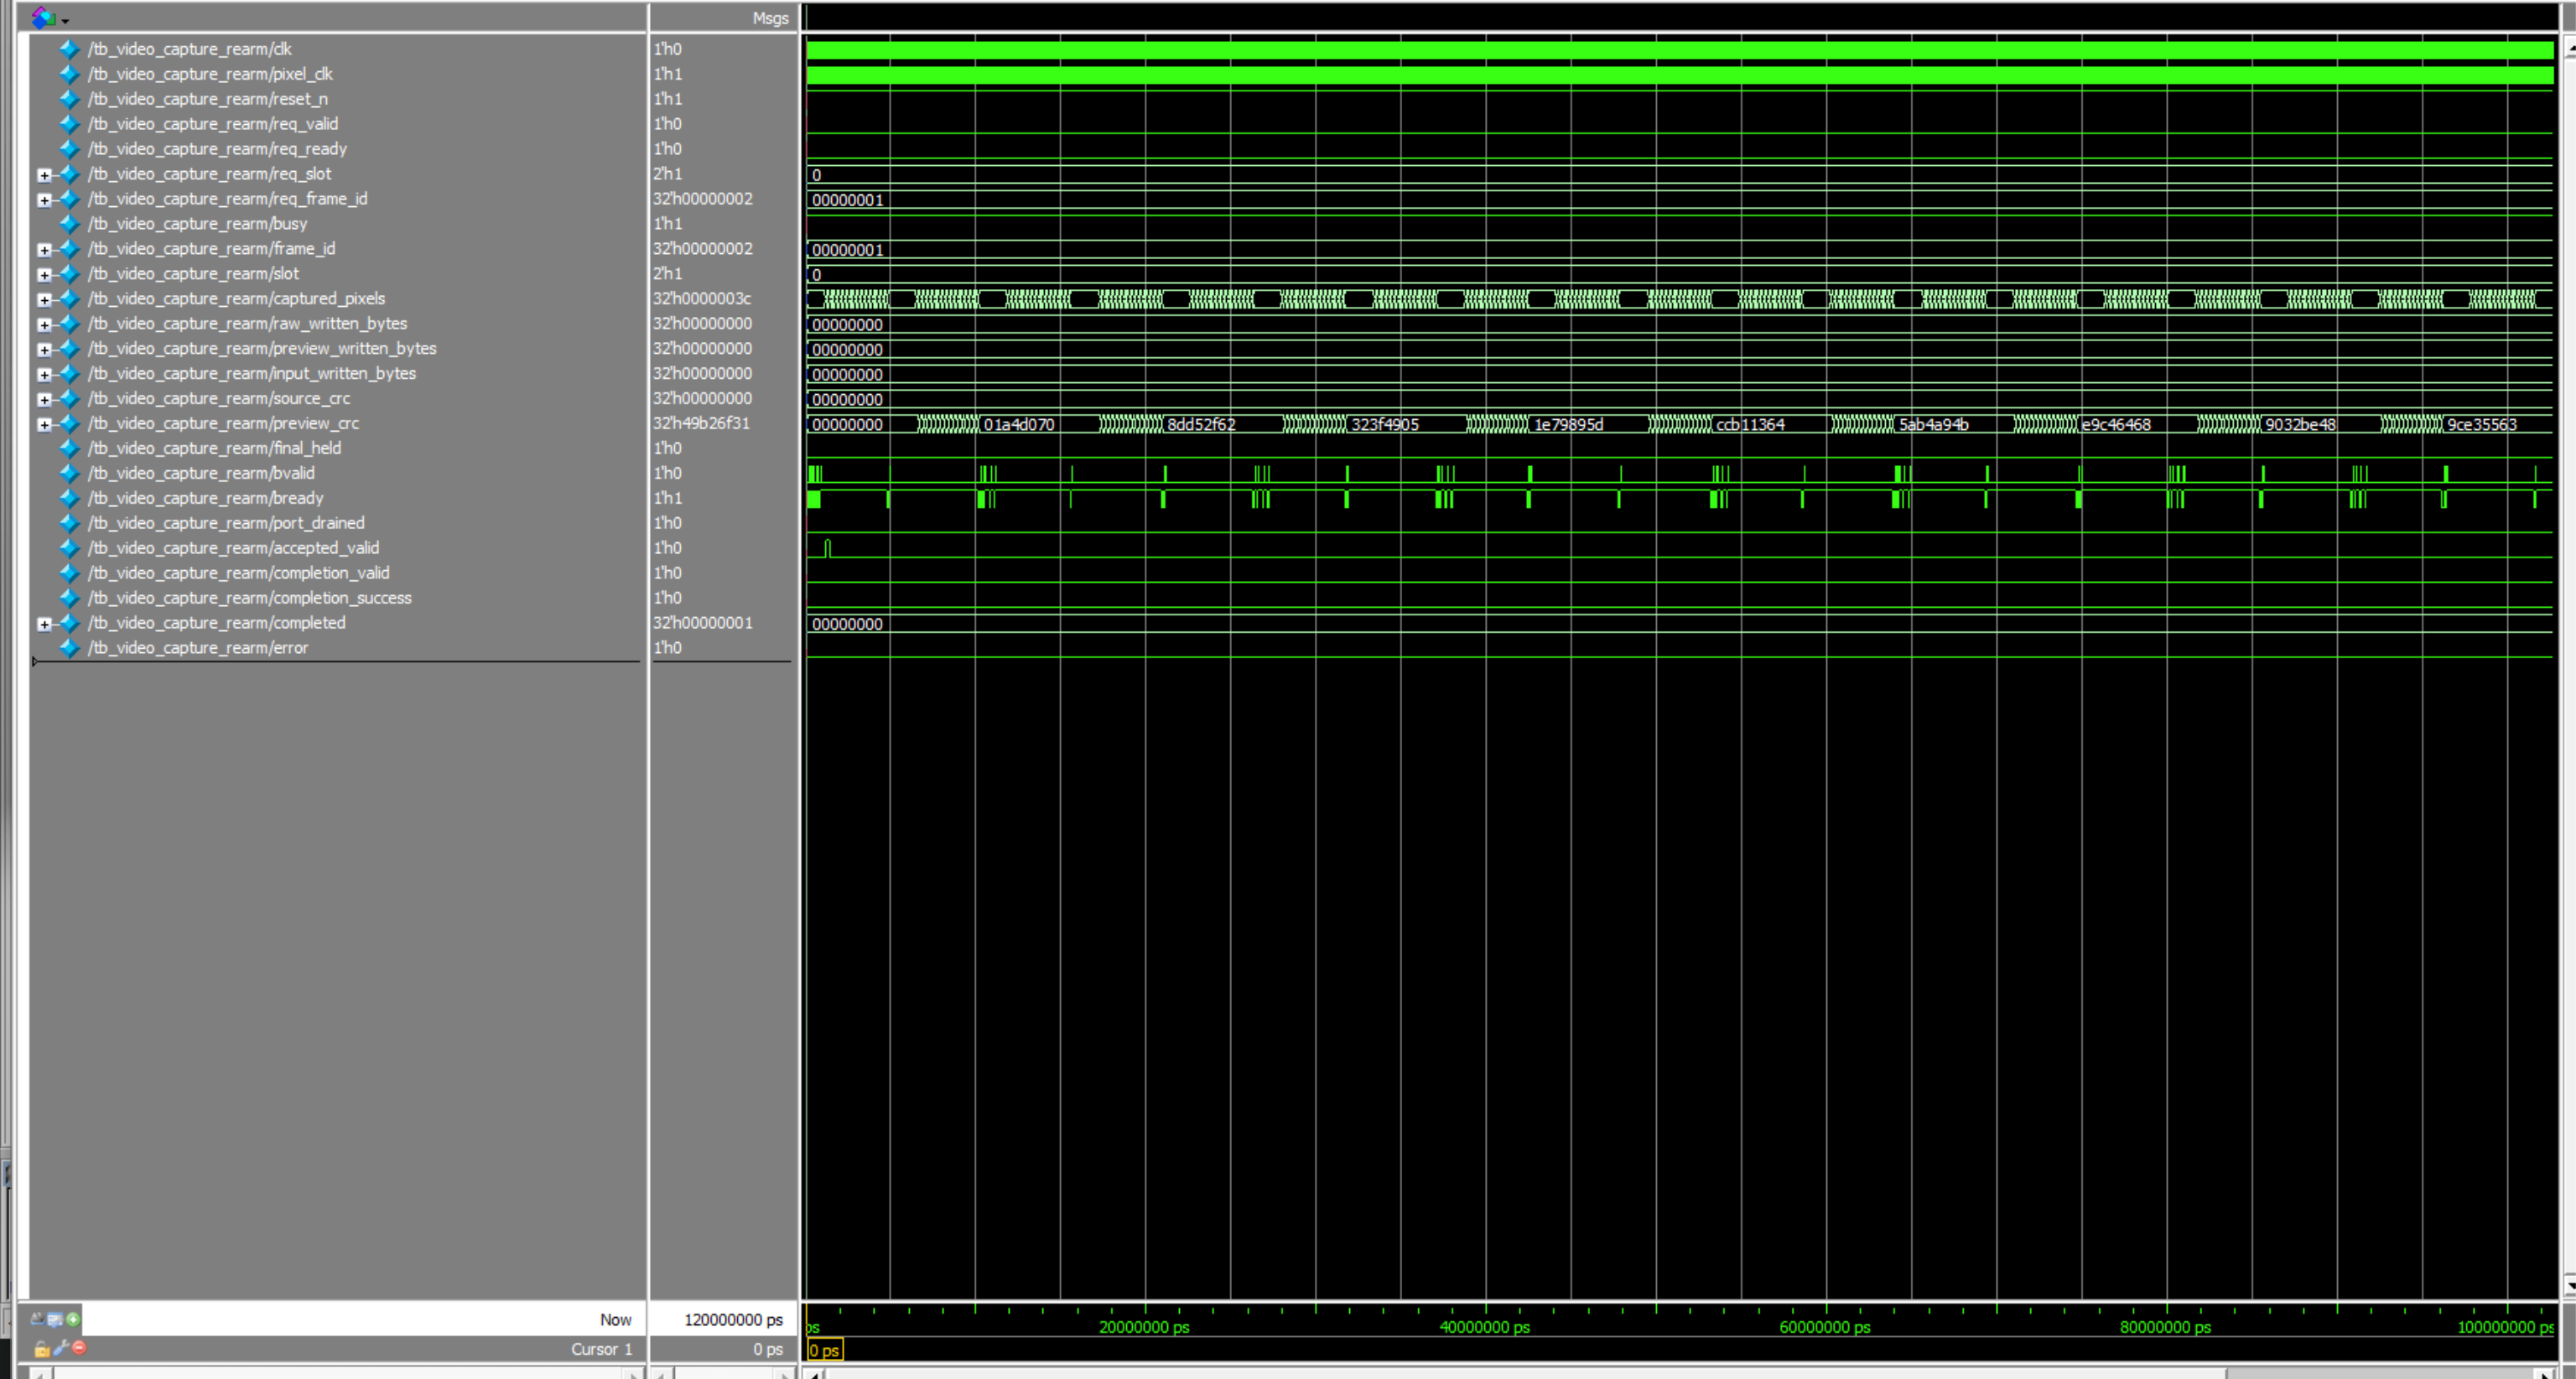
\includegraphics[width=0.8\linewidth]{../figure/video-capture-rearm-modelsim-native.png}
\caption{采集请求、三路写入计数、响应排空和完成事件波形}

\end{figure}

槽所有权场景将命令接收、显示生效和释放确认分开。\texttt{active\_\allowbreak slot\_\allowbreak o}及\texttt{active\_\allowbreak frame\_\allowbreak o}在匹配的显示反馈握手后更新；
旧槽依次进入RETIRING和等待释放确认状态，直至\texttt{release\_\allowbreak valid\_\allowbreak o}对应的释放握手完成才恢复为空闲。\texttt{protocol\_\allowbreak error\_\allowbreak o}全程为零。

\begin{figure}[!htbp]
\centering
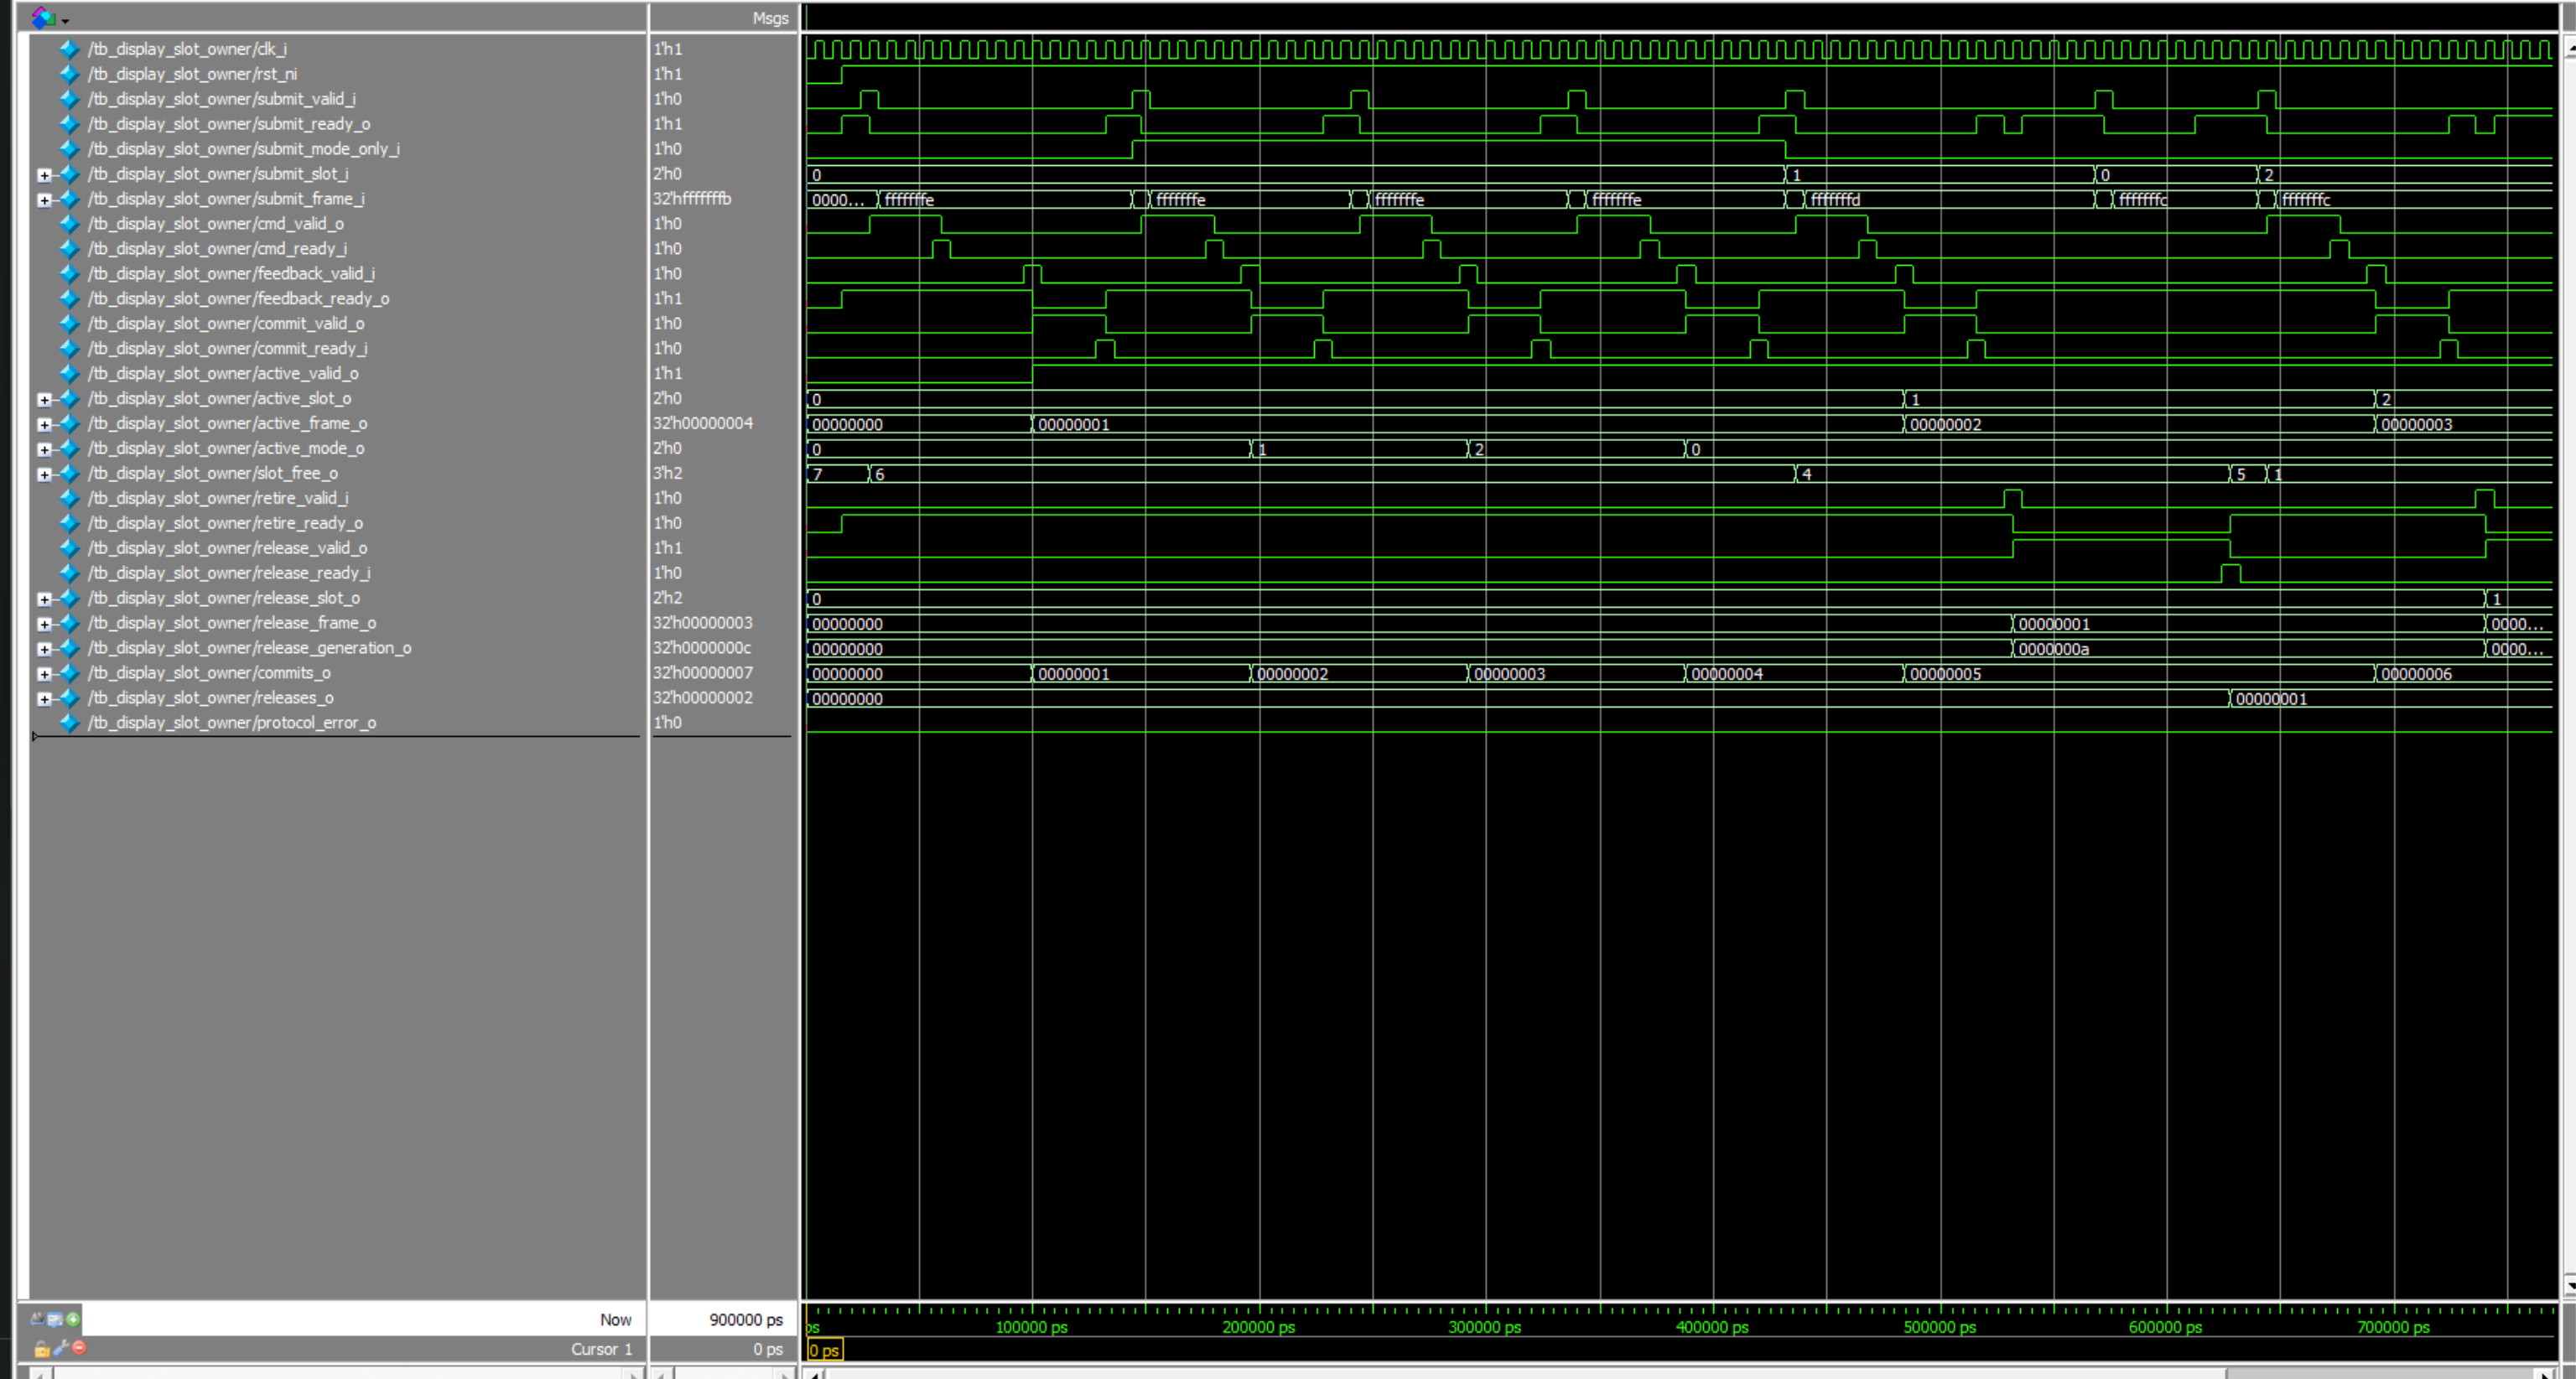
\includegraphics[width=0.8\linewidth]{../figure/video-slot-owner-modelsim-native.png}
\caption{显示槽提交、生效、代次和释放确认波形}

\end{figure}

\subsection{共享DDR背压与采显联合}

背压场景同时驱动写地址/写响应和读地址/读数据通道。波形显示读写通道分别被暂停时，仲裁器仍保持请求与发起端的对应关系，
\texttt{busy}和\texttt{port\_\allowbreak drained}在事务排空前不会提前结束；读写计数与测试台的12次读写请求一致。

\begin{figure}[!htbp]
\centering
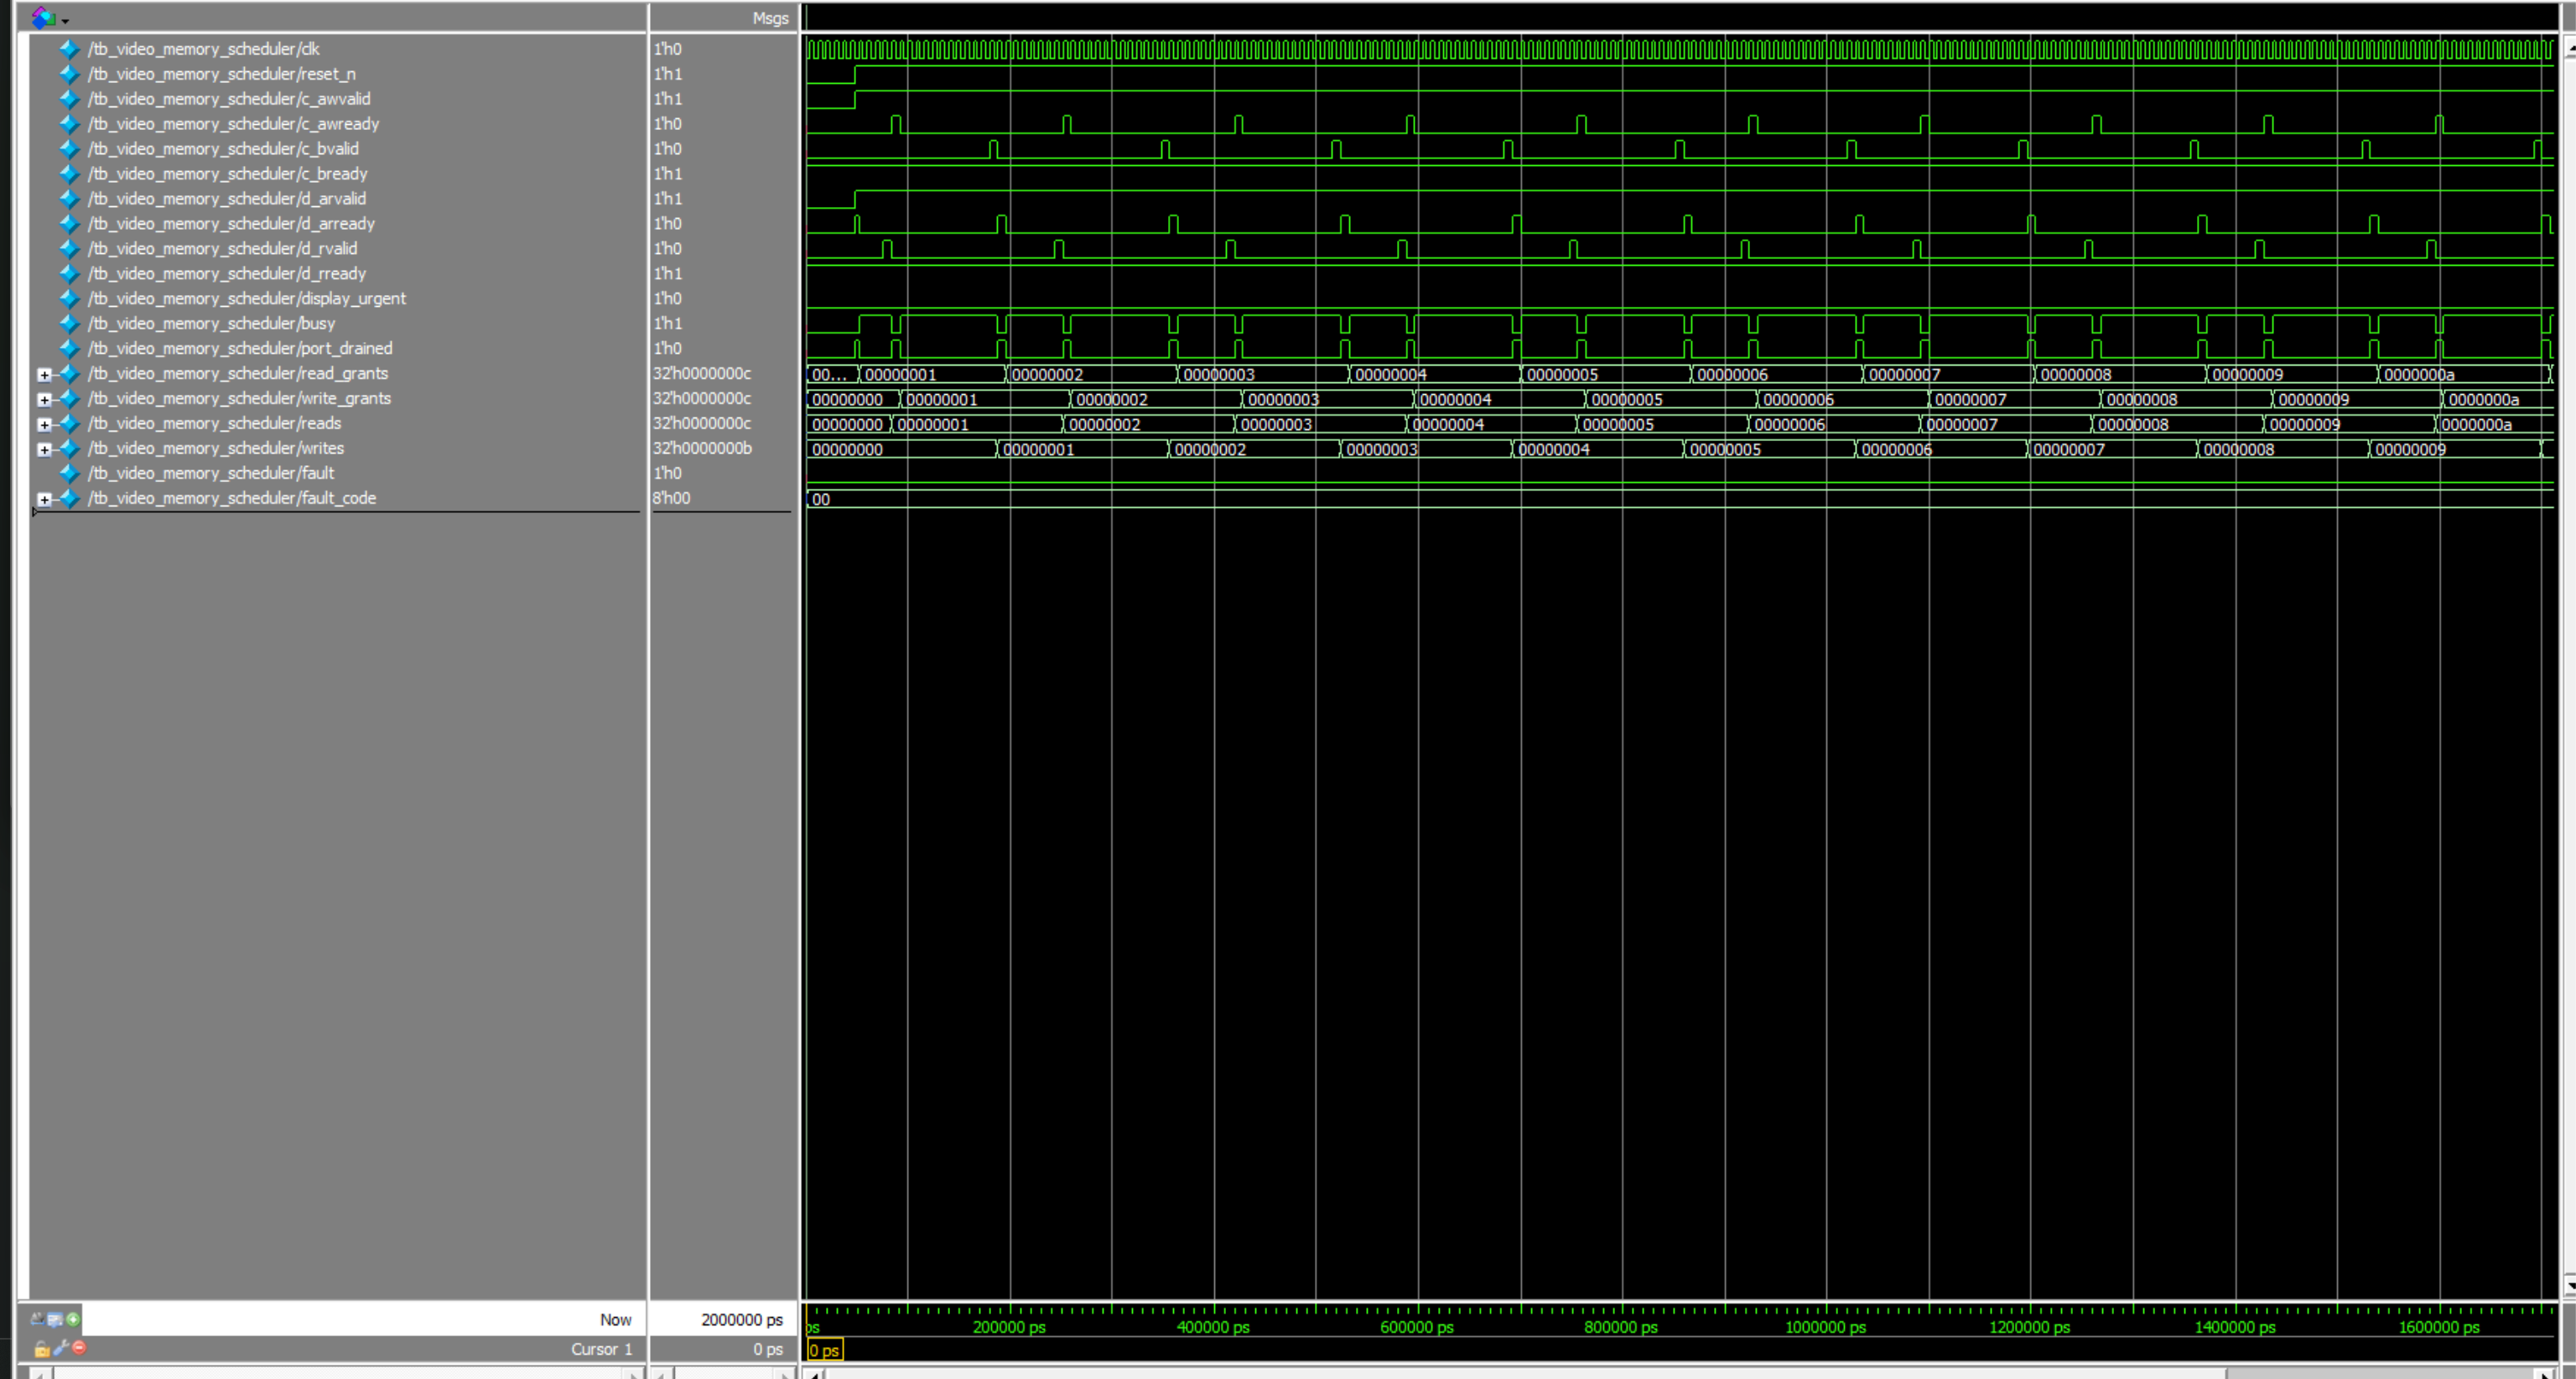
\includegraphics[width=0.8\linewidth]{../figure/video-ddr-backpressure-modelsim-native.png}
\caption{共享DDR读写握手、背压、仲裁计数和排空波形}

\end{figure}

联合场景把采集写、显示读、槽号及对应帧标识和像素输出放在同一时间轴上。
\texttt{commit\_\allowbreak frame\_\allowbreak id}、\texttt{release\_\allowbreak frame\_\allowbreak id}和\texttt{display\_\allowbreak frame}分别标记提交、释放和实际显示的帧标识，用于核对同一帧的事件顺序。
\texttt{underflows}保持为零，\texttt{seen\_\allowbreak commits}与\texttt{seen\_\allowbreak releases}按提交和释放事件推进，
\texttt{checked\_\allowbreak pixels}持续增加。2毫秒短窗口已经覆盖四个连续帧的提交/释放和采显重叠，完整13次光栅的数值结果见表\ref{tbl:video-high-value-sim}。

\begin{figure}[!htbp]
\centering
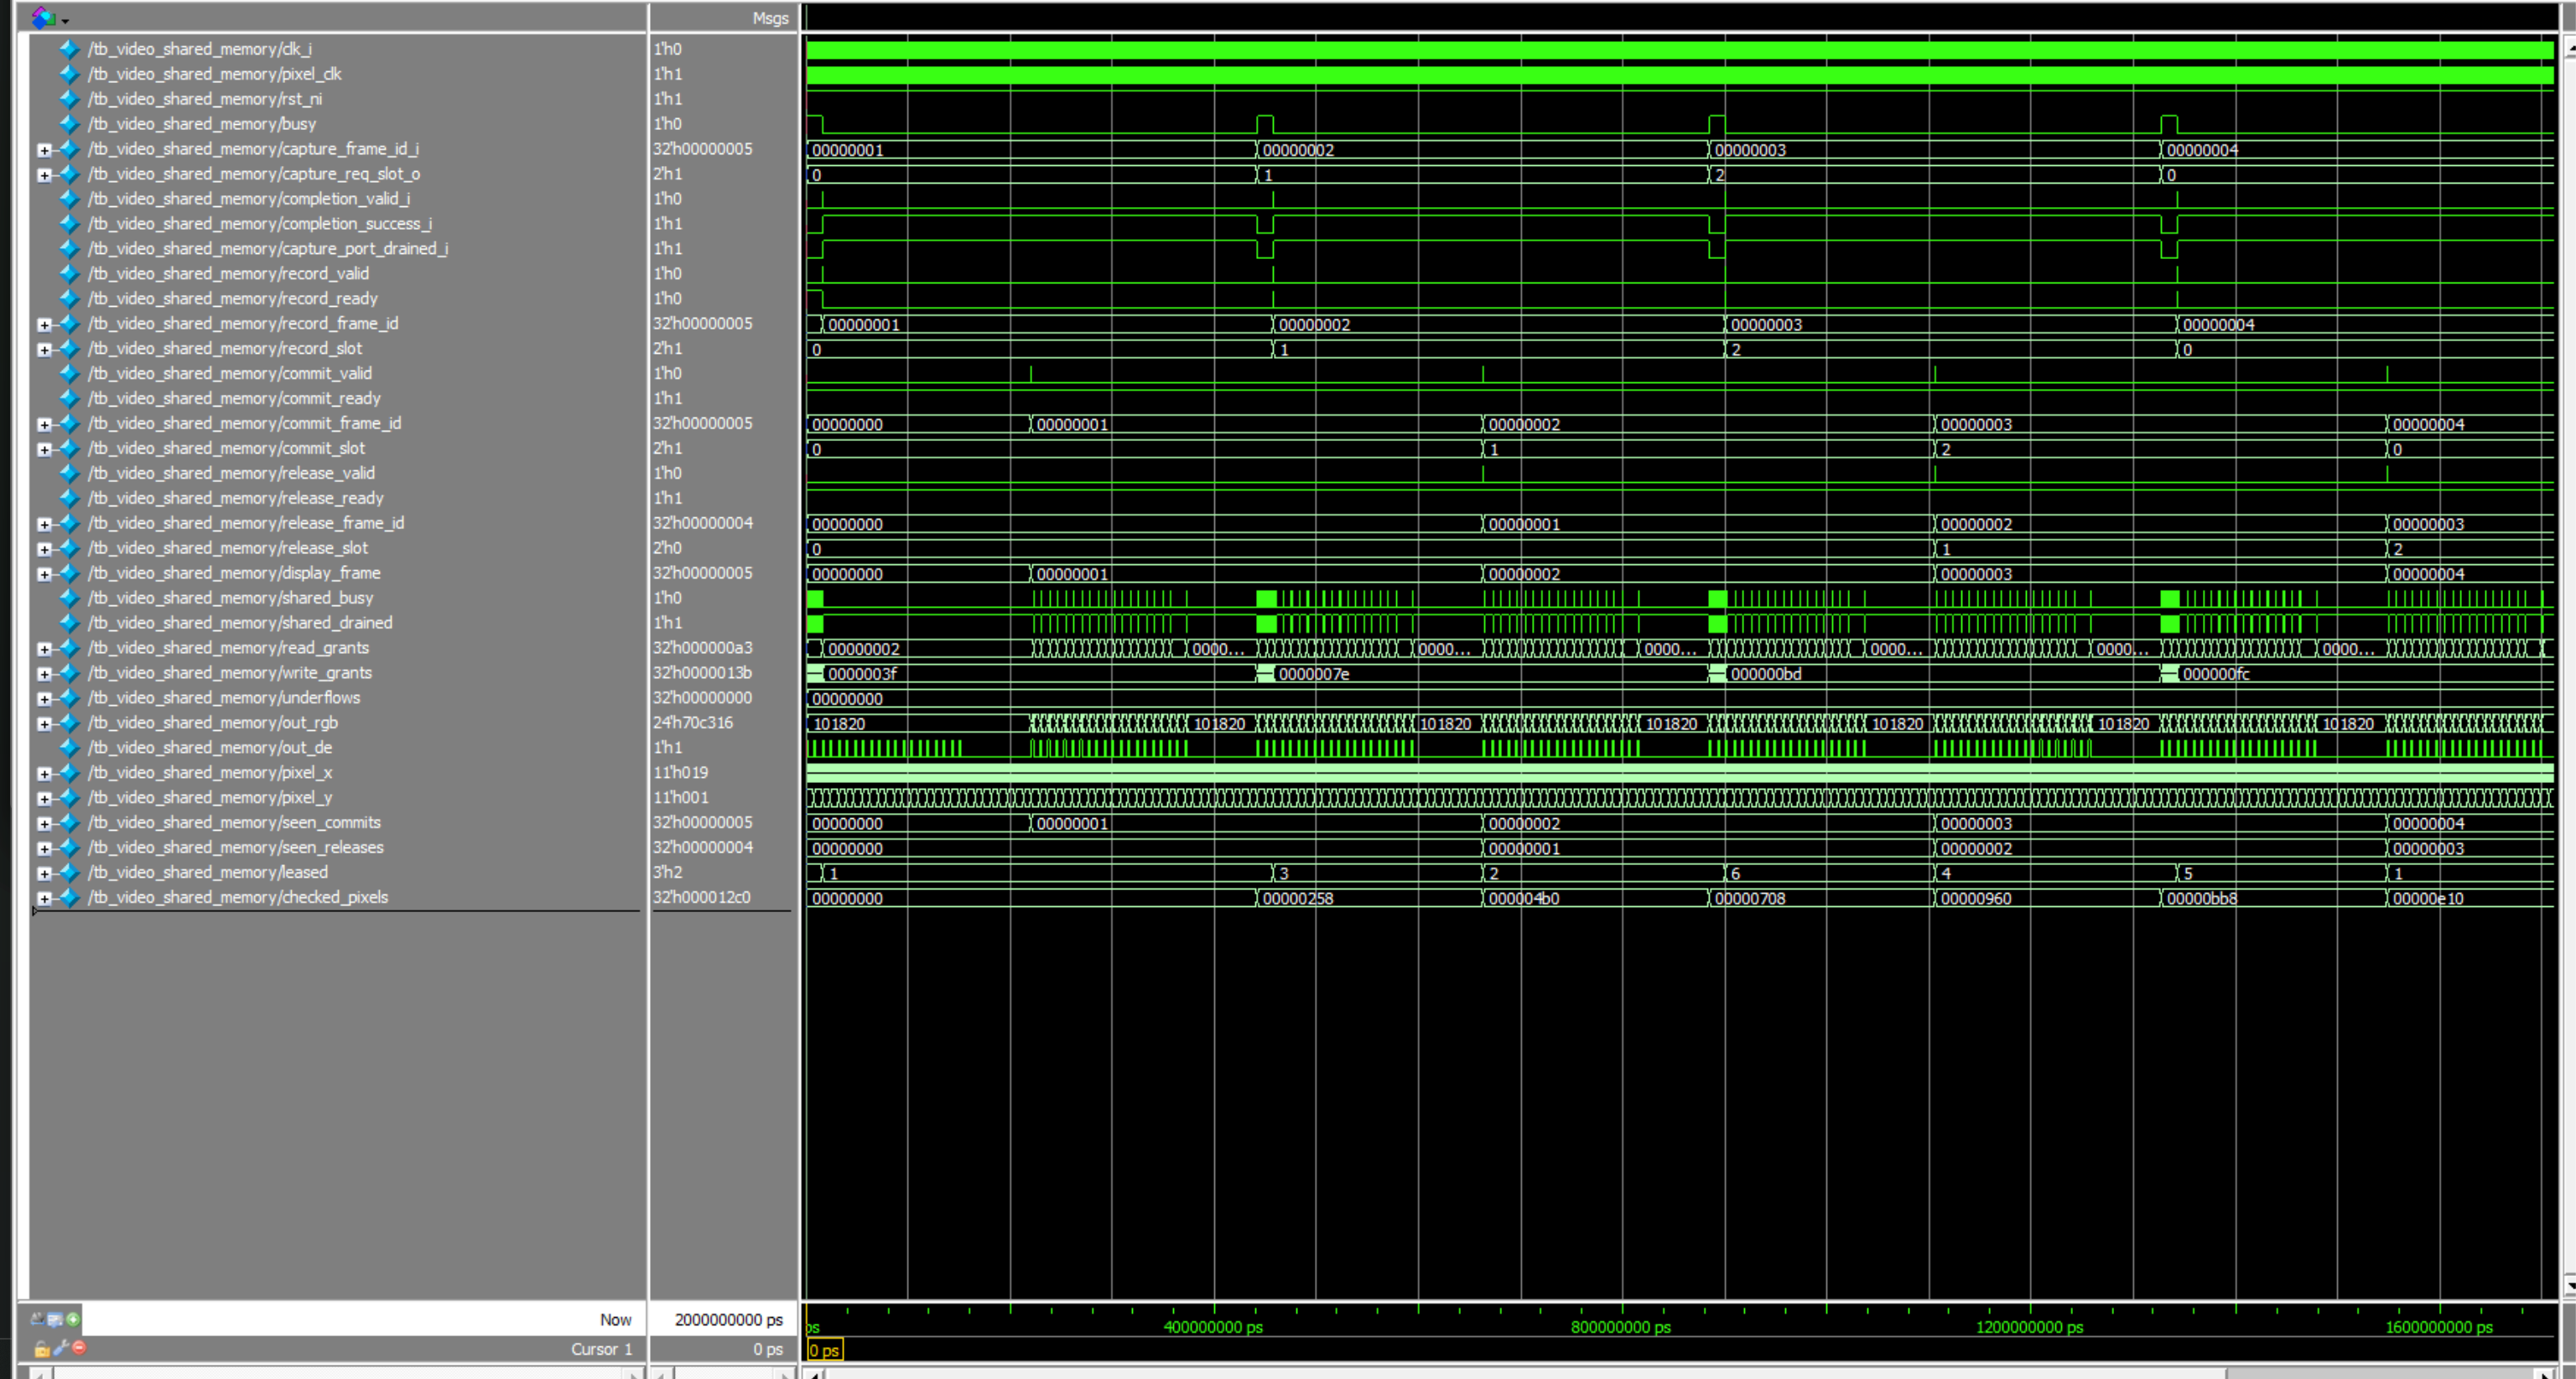
\includegraphics[width=0.8\linewidth]{../figure/video-shared-memory-modelsim-native.png}
\caption{采集、共享DDR、槽释放和像素输出联合波形}

\end{figure}

上述四类场景核对数字模型中的握手、所有权和背压传播，统计范围对应各自的组件测试；真实人脸检测应用的端到端功能由系统联合仿真及实板观测分别验证。

\subsection{紧凑显示组件回归}

紧凑显示接口在接收AXI-Lite读地址后先寄存请求，再执行译码。记录复制占用存储端口时，接口接收一项读请求并等待端口可用；
响应背压期间保持返回数据和响应码，复位时清除尚未完成的请求。MMIO回归检查接收地址保持、单项排队、响应稳定性及复位后的请求清除。
回归还检查显示命令接收后事件保持为零、实际像素反馈产生COMMIT，以及释放事件经ACK后更新空闲槽位图。

表\ref{tbl:video-compact-regression}列出紧凑显示接口的组件回归结果，原始配置与日志保存于\path{docs/verification/soc/face_box_report_20261103/}。
头像应用的完整采集、推理与三模式输出验证见附录\ref{sec:box-system-validation}。
27项为组件用例数，246项和1653项分别为记录检查与排队读用例内部的检查数。

\begin{reporttable}
\begin{longtable}{@{}>{\raggedright\arraybackslash}p{0.22\linewidth}p{0.16\linewidth}p{0.44\linewidth}p{0.10\linewidth}@{}}
\caption{紧凑显示组件回归结果}\label{tbl:video-compact-regression}\\
\toprule
测试范围 & 统计量 & 主要检查 & 结果 \\
\midrule
\endfirsthead
\caption[]{紧凑显示组件回归结果（续）}\\
\toprule
测试范围 & 统计量 & 主要检查 & 结果 \\
\midrule
\endhead
\bottomrule
\endfoot
显示组件回归 & 27项用例 & 显示接口、跨域交互与像素组合行为 & PASS \\
记录合法性检查 & 246项检查 & 显示记录格式、身份及边界条件 & PASS \\
MMIO排队读CASE10 & 1653项检查 & 复制占用时接收请求、地址保持、响应背压及复位 & PASS \\
\end{longtable}
\end{reporttable}

